\section{Preliminaries \& Running Example}
\label{sec:preliminaries}

This sections is structured as follows. First, we introduce the main concepts behind our approach, this is, the Design by Contract paradigm and security design pattern. Then, we describe in detail the \emph{Authenticator} pattern which will serve as a running example throughout the rest of the paper.

\subsection{Design by Contract}

The Design by Contract (DbC) concept was coined by Meyer \cite{meyer1992applying} as an approach to design reliable software based on the idea that elements of a software system collaborate with each other on the basis of mutual obligations and benefits, an so a contract between these elements.

Meyer indeed realized that the software systems, and in particular object-oriented systems, depend on the division of work. This means that tasks are classically divided in several sub-tasks, each being conducted by a software unit.

When this happens, the actual interaction of the units is entirely defined in a \emph{contract}. This contract contains the liabilities and benefits of the interaction for all parties involved. This analogy led Meyer to the idea of software contracting \cite{meyer1992applying}: to define contracts between clients (i.e., object’s callers) and suppliers (i.e., object functions or methods).

For software unit limited to a routine or method, a contract is defined as the aggregation of two assertions to this method:
\begin{itemize}
    \item A precondition:  Boolean condition that needs to be verified before executing the method. It summarizes the caller's obligations towards the supplier.
    \item A postcondition: Boolean condition that needs to be verified after the execution is made. It summarizes the supplier's obligations towards the caller.
\end{itemize}

In addition to these two assertions by method, Meyer defined a third type of Boolean expression called a \textit{class invariant}. This notion relies on the class concept, in object-oriented designs. A class is the representation of specific concept, usually defining its own objects or instances. Most of the time, a few properties characterize the essence of the class and should be true at all time and for every instance. A classic example of this idea, in a authentication process, a proof of identity must preserve its integrity, can't be updated. 

A proof of identity instance should verify at any time that its internal data can't be updated. This property is then an \textit{Invariant} for this class.
The whole idea of the DbC approach is that since a contract is formally defined for each unit (class) or module, bugs are unlikely to appear at run-time because of a misunderstanding between software units.



The DbC approach initially focused on software entities with limited scope, typically a class, was also extended to the notion of components \cite{beugnard1999,beugnard2010contract}.
We can also underline that this approach has been mainly used with the objective of software reliability in terms of software safety. 
The debug during the software development is the main interest of DbC. 

The security of software systems becoming a major concern at the moment, it seems relevant to evaluate this DbC approach, both in the design phase but also to guarantee a security contract during the execution.
Our objective is so to associate the Design by Contract with the Execution under Contract.

\subsection{Security Design Patterns}

In order to face the threats in terms of software security, security design patterns have naturally imposed themselves in the continuity of design patterns.
An abundant literature has been published, including books containing catalogs of patterns \cite{fernandezBooks}.

On the basis of these catalogs, different works have been developed to provide pattern languages in order to classify and create relations between patterns according to threats \cite{fernandez2013} or a formalization of patterns \cite{behrens2018} or specialized studies by domain like automotive for example \cite{cheng2019}.

Some works such as \cite{fernandez2018abstract} try to provide abstractions to the initial patterns in order to favor the expression of the semantics of the pattern. This abstract definition offers also the possibility to produce different more specialized patterns.  
We can note however that these abstract definitions respect the classical patterns approach and the expression of the solution remains on a structural definition based on a class diagram, certainly conceptual, and sequence diagrams for the behavioral part.

Like in \cite{fernandez2018abstract}, a security pattern is composed of several parts where mainly the problem, the solution and some additional comments are defined. These parts are deeply illustrated in the next section with the Authenticator pattern which is used throughout this paper to exemplify our approach and implementation.

\begin{comment}
\begin{itemize}
    \item The \emph{Intent}. This part describes in a few sentences the abstract intent of the pattern.
    \item The \emph{context}. The purpose is define the context to use the security pattern. 
    \item The \emph{problem}. This part describes the problem is addressed by the pattern.
    \item The \emph{forces}. This part lists several interested properties relative to the use of the pattern. Again this part is just a textual description

    \item The \emph{solution}. This part is usually composed of a UML (Unified Modeling Language) class diagram and a few sentences to explain the diagram.

    \item The \emph{remarks}. The authors of the pattern can add in this part any information they think is relevant. It usually involves performance results.
\end{itemize}


The following subsection presents the Authenticator pattern which is used throughout this paper to exemplify our approach and implementations.
\end{comment}

\subsection{The Authenticator pattern}

As defined in the previous section, the Authenticator pattern is characterized as follows:  
\begin{itemize}
    \item The \emph{Intent}. How to verify that a subject (user or system) intending to access the system is who it says it is? The subject must present information that is recognized by the system and is given some proof of the successful authentication.
    
    \item The \emph{context}. Computer systems contain sensible resources. We only want subjects that have some reason to be in our system to get into the system. 
    
    \item The \emph{problem}. The purpose is to prevent a malicious subject could try to impersonate a legitimate user to have access to the sensible resources. This could be particularly serious in case of the  impersonated user has a high level of privilege or offer the possibility to increase this level.

    \item The \emph{forces}. We emphasize some forces on this pattern:
    \begin{itemize}
        \item Authentication information protection. The pattern must assume the non-usurpation of the authentication information.
        % properties P1 and P2 and implicitly P3
        
        \item Authenticate authority integrity is preserve during its life to enforce the non-modification of the authentication information.
        % property P3 and implicitly P6
        
        \item Proof of identity tamper resistance. The integrity of the proof of identity presented by the user is preserved during its life-cycle.
        %Property P5 implicit P4
        
        \item Authentication process performance. Authentication should have a short response time or users will be annoyed and tried to bypass the authentication process.
        % Non property

        \item Authentication frequency. A user can't authenticate frequently in a given period of time. The purpose is to avoid many authentication tentative for a user or more annoying from security point of view, automatic attempts on the authenticate authority. 
        %P7     
    \end{itemize}

    This strengths list points to properties that must be respected to ensure proper use of the pattern.

    \item The solution. The solution definition includes a structural part and a behavioral one. The structural is generally express through a UML (Unified Modeling Language) class diagram like \ref{fig:authclasses}.
    
    Several entities are defined in this diagram:
    \begin{itemize}
        \item a \textit{Subject} needing to be authenticated,
        
        \item a \textit{Proof of Identity}, token given to the subject once the authentication is complete,
        
        \item an \textit{Authenticator} is the object which implements an authentication algorithm and creates the \textit{Proof of Identity},
        
        \item \textit{Authentication Information} are the information provided by the \textit{Subject} to the \textit{Authenticator}.
    \end{itemize}

The behavior definition is mainly based on several scenarios between the structural entities. These scenarios are illustrated through the code of our implementation, described in the section \ref{sec:case-study}.

    \item The \emph{remarks}. This last part is not detailed in this paper but usually the pattern authors add in this part any information they think is relevant. It usually involves performance results or customization aspects. 
\end{itemize}




\begin{figure}
    \centering
    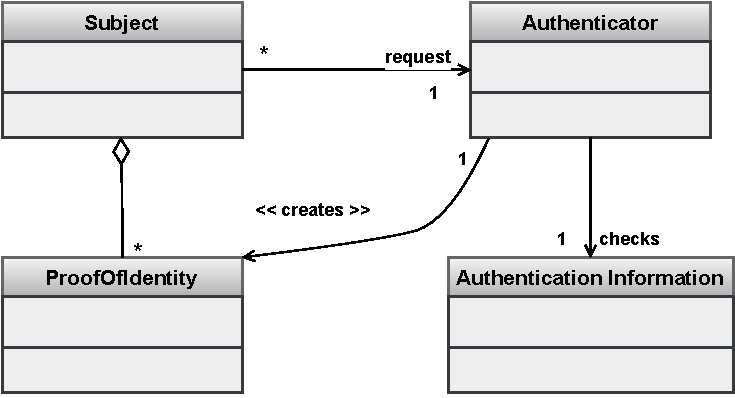
\includegraphics[width=0.7\columnwidth]{figures/AuthenticatorPattern.pdf}
    \caption{UML class diagram of the Authenticator pattern}
    \label{fig:authclasses}
\end{figure}

Based on this pattern, we will demonstrated how to create a security contract with related properties and how the implementation is independent and extensible of this defined contract. Trough the definition of the Authentication contract we emphasize the creation of a security harness on an existing code in weaving in it security aspects.
With our approach, we create also a link between the development process with the Design by Contract (DbC) and the Execution under Contract (EuC), to verify at run time the security properties.


%The goal of this pattern is to verify the identity of a subject. Such a subject can be someone interacting with a software by providing credentials, a subsystem requesting data to another subsystem, a thread requesting extra privilege to an operating system, etc. The pattern only provides an architecture which is compatible with the use of every authentication algorithm. The architecture of the Authentication pattern is presented in Figure \ref{fig:auth_classes}.


% Insister en conclusion sur comment créer un contrat de sécurité à partir de ce pattern et vérifier @run time que les prop de sécurité sont vérifiées qq soitr l'implantation.
% indépendance de l'implemenattion par rapport au contrat


%\subsection{Motivations} 

%\sm{We remove this subsection. Motivation is given at the end of 2.3. We say that the pattern is abstract and needs to be adapted and given more details in order for the pattern to be effective.}



%\begin{itemize}
%    \item Travailler avec du legacy code    
%   \item Pas seulement safety mais security pour gérer le truc qu'on ne sait pas prévoir
%    \item Dissocier les préoccupations fonctionnelles vs securité : aspect oriented programming (tissage @runtime)
%    \item Faire du monitoring@runtime avec un niveau de monitoring configurable
%    \item to associate the Design by Contract with the Execution under Contract.
%    \item Idée d'un "harnais" de sécurité au dessus d'un code fonctionnel
%    \item Idée de sécurisation de la composition de composants (eux-même peut-être déjà sécurisés): un contrat pour sécuriser le composition ?
%    \item besoin de fournir des implantations efficaces et démontrables des patterns cf article bib patterns, automotive ??
%\end{itemize}





